\chapter{凝视的控制} \label{chap:chap35}

在前面的章节中,我们了解了控制身体在空间中运动的运动系统。
在本章和下一章中,将探讨在我们在穿越周围世界时控制目光、平衡和姿势的运动系统。
在研究这些运动系统时,我们将重点关注这些系统解决的 3 个生物学挑战:
我们如何快速有效地从视觉上探索我们的环境?
我们如何补偿头部规划内和规划外运动?
我们如何保持直立?


在本章中,我们将描述动眼神经系统以及它如何使用视觉信息来引导眼球运动。
它是最简单的运动系统之一,只需要 12 块进化古老的肌肉来协调移动两只眼睛。
在人类和其他灵长类动物中,动眼神经系统的主要目标是控制中央凹的位置,中央凹是视网膜的中心点,感光细胞的密度最高,因此视力最敏锐。
中央凹的直径小于 1 毫米,覆盖的视野不到 1\%。
当我们想要检查一个物体时,我们必须将它的图像移动到中央凹上(第~\ref{chap:chap22}~章)。



\section{眼球被 6 块眼外肌所移动}

\subsection{眼球运动在眼眶中旋转眼球}

眼球一个很好的近似是一个位于眼眶中的球体。
眼球运动只是眼睛在眼眶中的旋转。
眼睛的方向可以由 3 个旋转轴(水平、垂直和扭转)定义,它们在眼球中心相交,眼球运动被描述为围绕这些轴的旋转。
水平和垂直眼球运动通过改变中央凹的方向来改变视线;
扭转眼球运动使眼睛围绕视线旋转,但不会改变眼睛注视的位置。


如图~\ref{fig:35_1}A~所示,眼睛远离鼻子的水平旋转称为\textit{外转},朝向鼻子的旋转称为\textit{内转}。 
垂直运动称为\textit{上转}(向上旋转)和\textit{下转}(向下旋转)。
最后,扭转运动包括\textit{内旋}(角膜顶部朝向鼻子旋转)和\textit{外旋}(远离鼻子旋转)。


\begin{figure}[htbp]
	\centering
	\includegraphics[width=1.0\linewidth]{chap35/fig_35_1}
	\caption{眼球运动的不同动作和控制它们的肌肉。
		A. 左眼视图和眼球运动的 3 个维度。
		B.1. 眼眶壁被切除的左眼侧视图。
		每块直肌(内直肌、外直肌、上直肌、下直肌)都插入眼球赤道的前方,因此收缩使角膜向肌肉旋转。
		相反,斜肌插入眼球赤道后面,收缩使角膜旋转远离插入点。
		上斜肌腱在插入眼球之前穿过滑车,滑车是眼眶鼻侧的骨滑轮。
		上眼睑的提肌抬起眼睑。
		2. 左眼俯视图,眼眶顶部和眼提肌被切除。 
		上直肌越过上斜肌并插入眼球前面。}
	\label{fig:35_1}
\end{figure}


大多数眼球运动是共轭的;
也就是说,两只眼睛以相同的方向和幅度移动,以维持单一的视觉图像。
这些眼球运动称为\textit{同向}运动。
例如,在向右凝视时,右眼外转而左眼内转。
同样,如果右眼外旋,左眼就会内旋。
当你的目光由远变近时,眼睛会向相反的方向移动:双眼内转。
这些运动称为\textit{聚散}运动。



\subsection{6 块眼外肌形成 3 个兴奋-拮抗对}

如图~\ref{fig:35_1}B~所示,每只眼睛由排列成 3 对主动-拮抗的 6 块眼外肌旋转。
4 块直肌(外直肌、内直肌、上直肌、下直肌)有一个共同的起点,即位于眼眶顶点的总腱环。
它们插入眼睛中心前面的眼睛表面或巩膜,因此上直肌抬高眼睛,下直肌压低眼睛。
下斜肌的起点在眼眶内侧壁上;
上斜肌的肌腱在插入眼球之前穿过滑车或滑车,因此它的有效起点也在眼眶的前内侧壁上。
斜肌插入眼睛中心的后方,因此上斜肌压低眼睛,下斜肌抬高眼睛。


每块肌肉都有双重插入。
离眼睛最远的肌肉部分插入软组织滑轮上,其余肌肉通过软组织滑轮到达眼睛。
当眼外肌收缩时,它们不仅会旋转眼睛,还会由于这些滑轮而改变其拉动方向。


眼外肌的动作由它们的几何形状和眼睛在眼眶中的位置决定。
内侧和外侧直肌水平旋转眼睛;
内直肌内收,而外直肌外展。
上直肌、下直肌和斜肌使眼睛在垂直方向和扭转方向上旋转。
上直肌和下斜肌抬高眼球,下直肌和上斜肌压低眼球。
上直肌和上斜肌进入眼睛,而下直肌和下斜肌外伸。


上直肌、下直肌和斜肌通常被称为旋垂直肌,因为它们产生垂直和扭转眼球旋转。
每次旋转的相对量取决于眼睛位置。
如图~\ref{fig:35_2}~所示,上直肌和下直肌在眼球外转时发挥最大垂直作用,即视线与肌肉牵拉方向平行时,而斜肌在眼球内转时发挥最大垂直作用。


\begin{figure}[htbp]
	\centering
	\includegraphics[width=0.66\linewidth]{chap35/fig_35_2}
	\caption{眼眶位置对上斜肌活动的影响。
		A. 当眼睛内收(朝鼻子看)时,上斜肌的收缩使眼睛下转。
		B. 当眼睛外转时(从鼻子向外看),上斜肌收缩使眼睛内旋。}
	\label{fig:35_2}
\end{figure}



\subsection{两只眼睛的运动是协调的}

人类和其他眼睛在前的动物具有双眼视觉(两只眼睛的视野重叠)。
这有助于立体视觉,即在 3 个维度上感知视觉场景的能力,以及深度感知。
同时,双眼视觉需要两只眼睛运动的精确协调,使 2 个中央凹始终对准感兴趣的目标。
对于大多数眼球运动,双眼必须以相同的量和相同的方向移动。 
这在很大程度上是通过两只眼睛的眼部肌肉配对来实现的。


正如每块眼肌都与其在同一眼眶中的拮抗肌配对(例如,内侧和外侧直肌)一样,它也与在相同方向上移动对侧眼睛的肌肉配对。
例如,在向左\textit{眼跳}期间,左侧外直肌和右侧内直肌的耦合使双眼向左移动。
垂直肌的方向是这样的,每对由一根直肌和一根斜肌组成。
例如如表~\ref{tab:35_1}~所示,左上直肌和右下斜肌在左眼注视时均使眼睛向上移动,而右下直肌和左上斜肌在右眼注视时均使眼球向下移动。


\begin{table}[htbp]
	\caption{内转和外转中的垂直肌肉动作\label{tab:35_1}}
	\centering
	\begin{tabular}{ccc}
		\toprule
		肌肉 & 内转的动作 
		& 外转的动作 \\
		\midrule
		上直肌 & 内旋  & 上转 \\
		下直肌      & 外旋 	& 下转 \\
		上斜肌      & 下转 	& 内旋 \\
		下斜肌      & 上转 	& 外旋 \\
		\bottomrule
	\end{tabular}
\end{table}



\subsection{眼外肌由 3 对颅神经控制}

如图~\ref{fig:35_3}~所示,眼外肌由位于脑干特定核团中的运动神经元组支配,运动神经元的细胞体聚集在脑干的 3 个动眼神经核中。
外直肌由外旋神经(第 VI 颅神经)支配,外旋神经的核位于第四脑室底部的脑桥中。
上斜肌受滑车神经(第 IV 颅神经)支配,滑车神经核位于对侧中脑下丘水平\footnote{滑车神经得名于滑车,即上斜肌穿过的骨滑轮。}。


\begin{figure}[htbp]
	\centering
	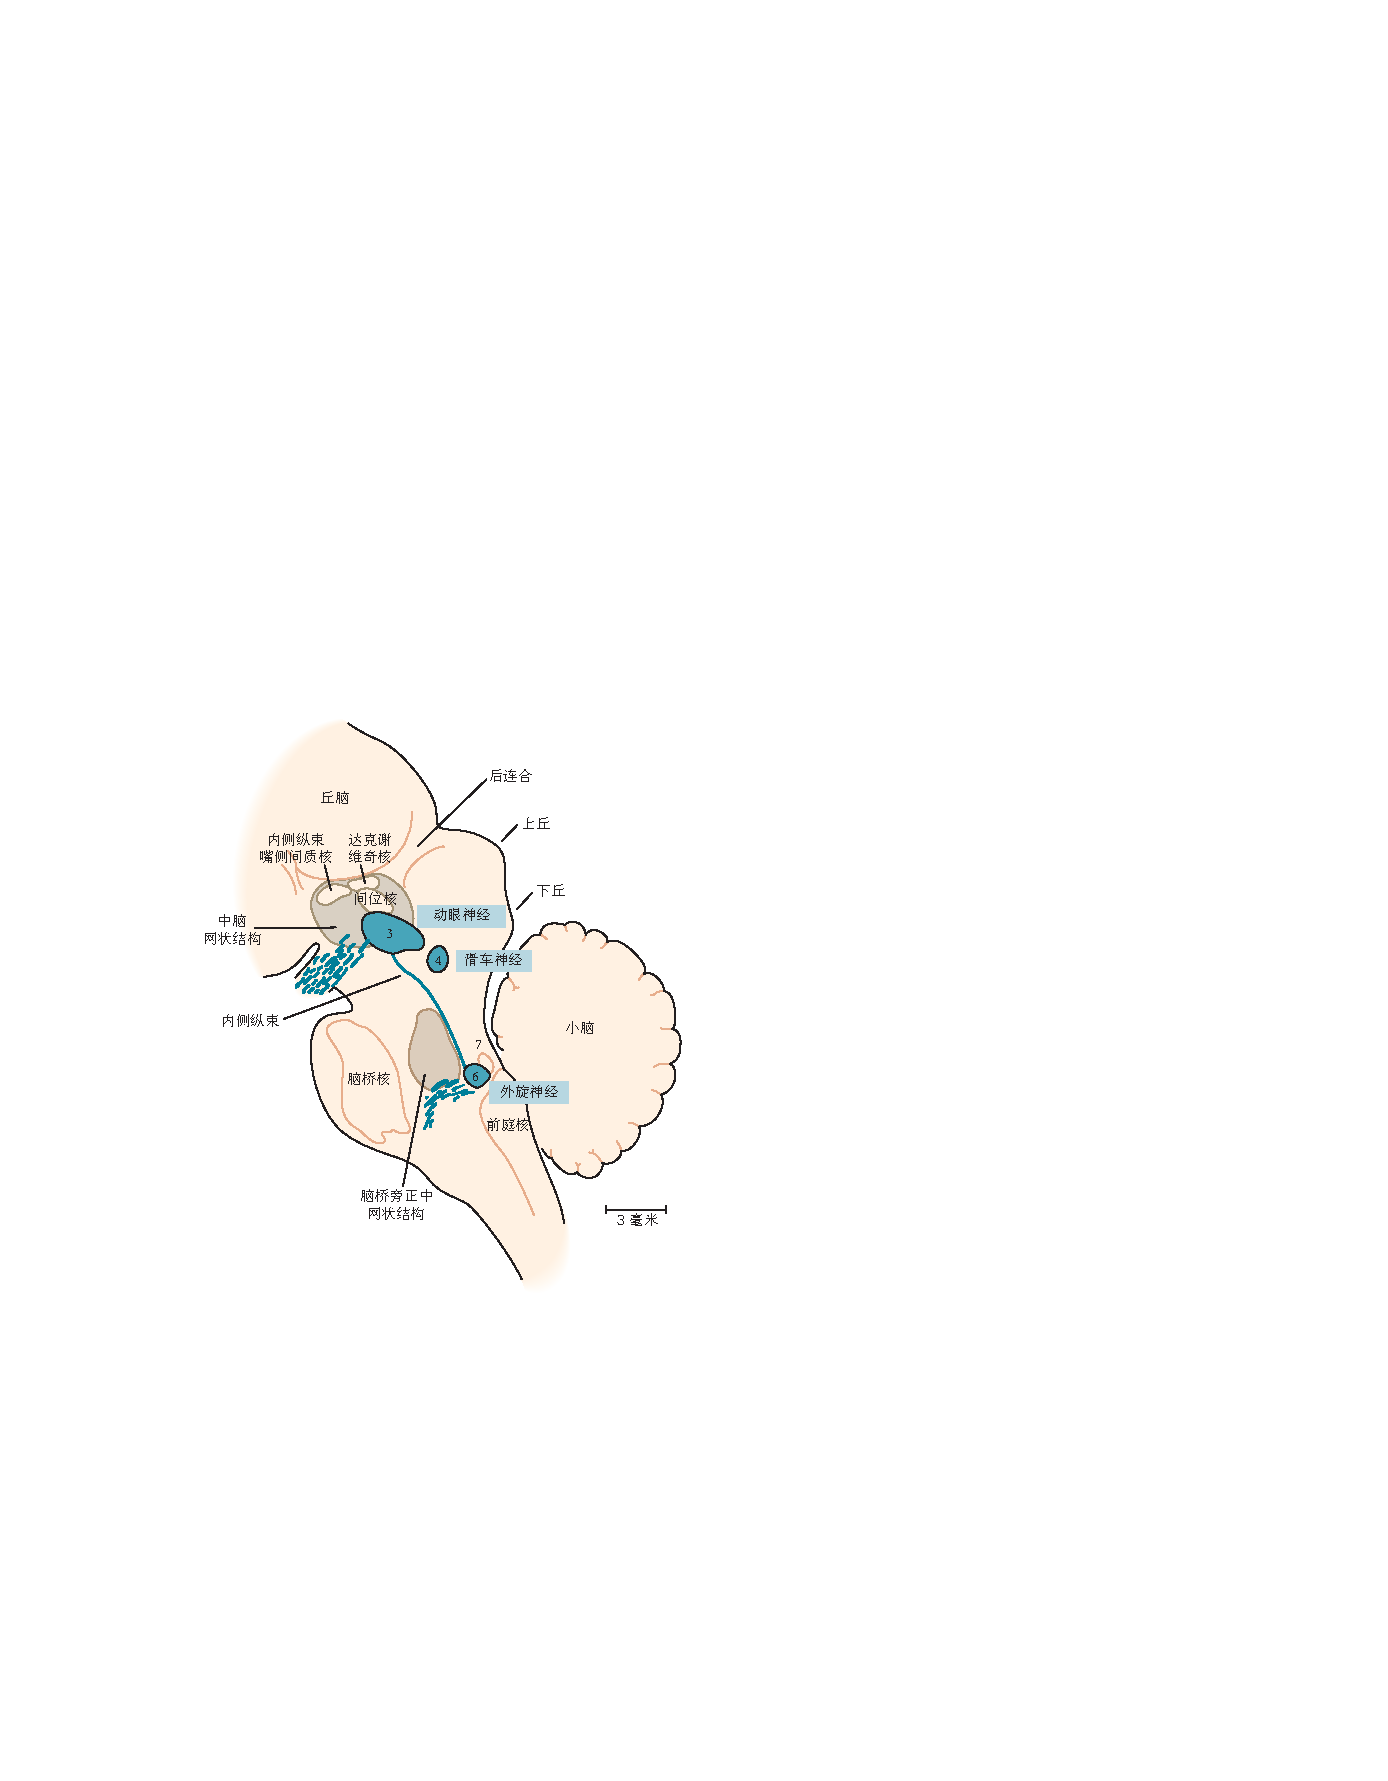
\includegraphics[width=0.62\linewidth]{chap35/fig_35_3}
	\caption{脑干中的动眼神经核。
		细胞核显示在恒河猴的丘脑、中脑、脑桥和小脑的矢状旁切面中。
		动眼神经核(第 3 颅神经)位于中脑中脑网状结构水平;
		滑车神经核(第 4 颅神经)略微位于尾部;
		外旋神经核(第 6 颅神经)位于\textit{脑桥旁正中网状结构}水平的脑桥,与面神经(第 7 颅神经)的束相邻\cite{henn1982primate}。
		与图~\ref{fig:40_5}~进行比较。}
	\label{fig:35_3}
\end{figure}


其他所有眼外肌(内直肌、下直肌、上直肌和下斜肌)由动眼神经(第 3 颅神经)支配,其核位于中脑上丘水平。
上直肌轴突穿过中线并加入对侧动眼神经。
因此,上直肌和上斜肌运动神经元支配它们各自对侧的肌肉。
动眼神经还包含支配眼提肌的纤维。
支配双眼睑的轴突细胞体位于中央尾核,这是动眼神经复合体中的单个中线结构。
最后,与动眼神经一起移动的是支配虹膜括约肌和睫状肌的副交感神经纤维,虹膜括约肌会收缩瞳孔,睫状肌会在从远到近的聚散运动过程中调整晶状体的曲率以聚焦眼睛,即调节过程。


瞳孔和眼睑也有交感神经支配,起源于同侧上胸段脊髓的中间外侧细胞柱。
这些神经元的纤维与上颈部的颈上神经节细胞形成突触。
这些节后细胞的轴突沿着颈动脉行进到海绵窦,然后进入眼眶。
交感神经瞳孔纤维支配虹膜扩张肌,导致瞳孔扩张,这是“战斗或逃跑”响应的一部分。
交感神经纤维还支配米勒肌,这是上眼睑的二级提拉肌。
瞳孔扩张和眼睑抬高的交感神经控制是兴奋和交感神经超负荷的“睁大眼睛”表情的原因。



观察特定神经损伤后的眼球运动是了解眼外肌活动的最佳方法(文本框~\ref{box:35_1})。


\begin{proposition}[眼外肌肉或神经损伤] \label{box:35_1}

\quad \quad 患有眼外肌肉或其神经病变的患者抱怨复视,因为凝视对象的图像不再落在双眼的相应视网膜位置上。
每种神经的损伤都会产生典型症状,这取决于哪些眼外肌肉受到影响。
一般来说,当患者试图朝着虚弱肌肉的方向看时,复视会增加。


\quad \quad \textbf{外旋神经}

\quad \quad 外旋神经(第 6 对颅神经)损伤导致外直肌无力。
当病变完全时,眼睛不能外展超过中线,因此当受试者朝受影响眼睛的方向看时,水平复视会增加。


\quad \quad \textbf{滑车神经}

\quad \quad 如图~\ref{fig:35_4}~所示,左滑车神经(第 4 颅神经)损伤通过削弱上斜肌影响扭转和垂直眼球运动。
上斜肌麻痹的垂直错位也受到头部位置的影响。
向一侧倾斜,使耳朵向肩膀移动,会引起眼睛向相反方向的小扭转,称为眼球反侧滚动。
例如,当头部向左倾斜时,左眼通常由左上直肌和左上斜肌发音,而右眼则由右下直肌和右下斜肌发音。
在左眼中,上直肌的抬高动作被上斜肌的下压动作抵消,因此眼睛只围绕视线旋转。
当头部向右倾斜时,下斜肌和下直肌压迫左眼,上斜肌和上直肌放松。


\quad \quad 在左上斜肌麻痹的情况下,当头部向左倾斜以使左眼进一步向上移动时,上直肌的抬高作用是不受阻碍的。
相反,如图~\ref{fig:35_4}~所示,头部向右倾斜可以放松上直肌和上斜肌。
因此,滑车神经病变的患者通常更喜欢将头部倾斜远离受影响的眼睛,因为这可以减少错位并消除复视。


\quad \quad \textbf{动眼神经}

\quad \quad 动眼神经(第 3 颅神经)的损伤具有复杂的影响,因为该神经支配多块肌肉。
一个完整的损伤只保留外侧直肌和上斜肌。
因此,瘫痪的眼睛通常向下偏斜,在休息时被绑架,不能向内侧或向上移动。
向下运动也会受到影响,因为下直肌较弱;
由于眼睛是被诱拐的,完整的上斜肌的主要作用是内翻而不是凹陷。


\quad \quad 由于控制眼睑抬高、调节和瞳孔收缩的纤维在动眼神经中传播,对该神经的损伤也会导致眼睑下垂(上睑下垂)、近距离物体视觉模糊和瞳孔扩张(散瞳)。
尽管交感神经支配在动眼神经损伤的情况下仍然完整,但上睑下垂基本上是完全的,因为\textit{米勒肌}对上眼睑抬高的贡献小于上眼睑提肌。


\quad \quad \textbf{交感眼动神经}

\quad \quad 支配眼睛的交感神经纤维来自胸脊髓,穿过肺尖,在颈动脉外侧上行到眼睛。
通往眼睛的交感神经通路中断会导致\textit{霍纳综合症},包括由于米勒肌无力导致的部分同侧上睑下垂和同侧瞳孔相对收缩(瞳孔缩小)。
瞳孔不对称在弱光下最为明显,因为正常瞳孔可以扩张,但受\textit{霍纳综合症}影响的瞳孔则不能。
	
\end{proposition}


\begin{figure}[htbp]
	\centering
	\includegraphics[width=0.78\linewidth]{chap35/fig_35_4}
	\caption{左滑车神经麻痹的疗效。
		滑车神经支配上斜肌,上斜肌插入眼球赤道后方。
		当它内收时,它会压低眼睛,当它外转时,它就会内旋眼睛。
		A. 斜视是一种眼睛的永久性向上偏斜,当患者直视前方时可以看到。
		右眼位于眼眶中心,但受影响的左眼略高于右眼。
		B. 当眼睛内收时,由于无阻扰的下斜肌将眼睛推高(左),因此斜视更严重。
		当眼睛被诱拐(右)时,情况会得到改善,因为上斜肌对凹陷的贡献小于对内翻的贡献。
		C. 当患者向右看时,斜视向下看(左)比向上看(右)更严重。
		D. 头向右(左)倾斜可改善高渗,向左(右)倾斜可恶化。
		眼球反滚动反射引起左眼向左倾斜时的内斜视和眼睛向右倾斜时的外斜视(第~\ref{chap:chap27}~章)。
		头向左倾斜时,内翻需要增加上直肌的活动,上直肌的提升活动不受弱上斜肌的影响,从而导致高斜视增加。
		随着头部向右倾斜和左眼外展,无对手的上直肌活动减少,斜视减少。}
	\label{fig:35_4}
\end{figure}


眼外肌产生的力取决于运动神经元的放电频率以及它们所募集的运动单位的数量,这是神经控制眼球运动精细调节的一部分。
与骨骼肌的运动单位(第~\ref{chap:chap31}~章)一样,眼球运动单位以固定顺序募集。
例如,当眼睛横向移动时,活跃的外旋神经元数量及其个体放电率都会增加,从而增加外直肌收缩的强度。



\section{6 种神经元控制系统保持目标的瞄准}

动眼神经核是高层大脑网络产生的所有类型眼球运动的最终共同目标。
\textit{赫尔曼$\cdot$亥姆霍兹}和其他 19 世纪的心理物理学家认为,眼球运动分析对于理解视觉感知至关重要,但他们假设所有眼球运动都是平滑的。
1890 年,\textit{爱德华$\cdot$兰德}发现,在阅读过程中,眼睛不会沿着一行文字平稳移动,而是会快速间歇性地移动,称为\textit{眼跳},每次\textit{眼跳}后都有一个短暂的停顿。


到 1902 年,\textit{雷蒙德$\cdot$道奇}概述了 5 种不同类型的眼球运动,它们将中央凹引导至视觉目标并将其保持在那里。
所有这些眼球运动都共享一个效应通路,该通路起源于脑干中的 3 个动眼神经核。


\textit{眼跳}迅速将中央凹转移到新的视觉目标。


\textit{平滑跟踪}运动将移动目标的图像保持在中央凹上。


聚散运动使眼睛朝相反的方向移动,因此无论距离多远,感兴趣的物体的图像都位于 2 个中央凹上。


\textit{前庭-眼动反射}在短暂的头部运动期间稳定视网膜上的图像。


视动运动在持续的头部旋转或平移过程中稳定图像。


第 6 个系统(即注视系统)在头部不动时通过主动抑制眼球运动使眼睛保持静止。
视动系统和前庭系统在第~\ref{chap:chap27}~章中讨论。
我们在这里考虑其他 4 个系统。



\subsection{主动固定系统使中央凹保持对静止目标的注视,以实现准确的视线定位。}

当眼睛静止时,视力最准确。
当我们检查感兴趣的对象时,凝视系统会主动防止眼睛移动。
当我们做一些不需要视觉的事情时,比如心算,它就不会那么积极地抑制运动。
注视系统障碍的患者(例如,无法抑制\textit{眼跳}的患者,即视阵挛),视力不佳不是因为他们的视敏度不足,而是因为他们不能保持眼睛足够静止以使视觉系统正常工作。



\subsection{\textit{眼跳}系统将中央凹指向感兴趣的对象}

如图~\ref{fig:35_5}~和第~\ref{chap:chap25}~章所示,我们的眼睛通过一系列非常快速的\textit{眼跳}探索世界,这些\textit{眼跳}将中央凹从一个注视点移动到另一个注视点。
\textit{眼跳}使我们能够快速扫描环境并阅读。 
他们有一个高度定型的标准波形,眼速度有一个平滑的增加和减少。
如图~\ref{fig:35_6}A~所示,\textit{眼跳}也非常快,在几分之一秒内以高达每秒 900° 的角速度发生。
\textit{眼跳}的速度仅由其大小决定。
我们可以自主改变\textit{眼跳}的幅度和方向,但不能改变\textit{眼跳}的速度,尽管疲劳、药物或病理状态会减慢\textit{眼跳}。


\begin{figure}[htbp]
	\centering
	\includegraphics[width=0.5\linewidth]{chap35/fig_35_5}
	\caption{眼球运动跟踪关注对象的轮廓。
		观察者注视一张女性照片 1 分钟。
		然后将得到的眼睛位置叠加在图片上。
		如图所示,观察者专注于脸部的某些特征,在女士的眼睛和嘴巴上逗留(注视),而在中间位置花费较少的时间。
		视点之间的快速移动是\textit{眼跳}\cite{yarbus2013eye}。}
	\label{fig:35_5}
\end{figure}


\begin{figure}[htbp]
	\centering
	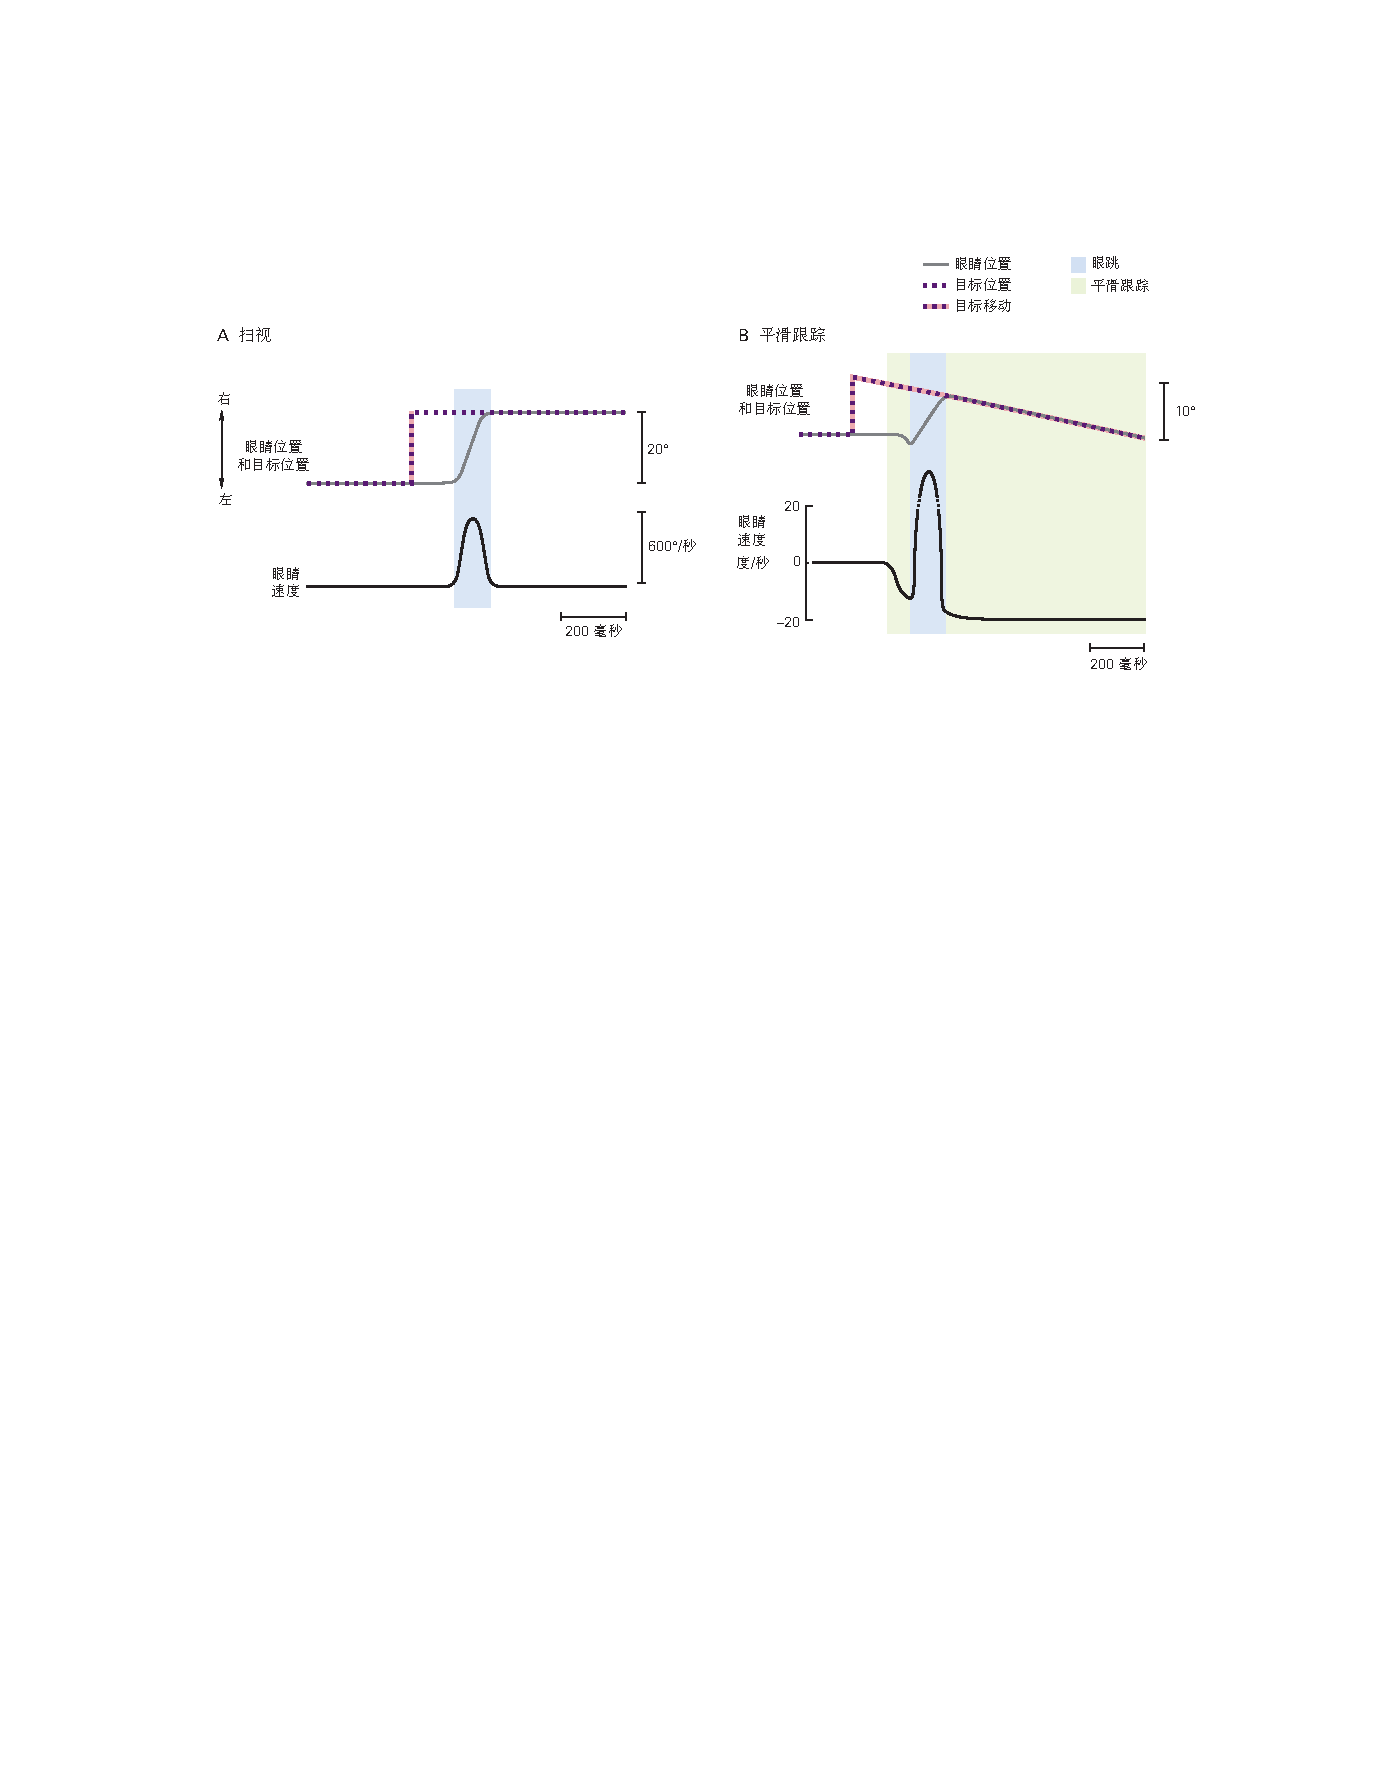
\includegraphics[width=1.0\linewidth]{chap35/fig_35_6}
	\caption{\textit{眼跳}和平滑的眼球运动。
		眼睛位置、目标位置和眼睛速度随时间绘制。
		A. 人类的\textit{眼跳}。
		在曲线图的开始,眼睛在目标上(代表眼睛和目标位置的轨迹是叠加的)。
		突然目标向右跳,在 200 毫秒内,眼睛移动将目标带回中央凹。
		请注意平滑、对称的\textit{眼睛速度}曲线。
		因为眼球运动是眼球在眼眶内的旋转,所以用旋转角度来描述。
		类似地,视野中的物体通过它们对着眼睛的弧度来描述。
		从手臂的长度看,拇指所夹的角度大约为 1°。
		因此,从拇指的一个边缘到另一个边缘的\textit{眼跳}穿过 1° 的弧度。
		B. 人类的\textit{平滑跟踪}。
		在这个示例中,受试者被要求对一个目标进行\textit{眼跳},该目标从注视中心跳开,然后慢慢移回中心。
		在位置和速度轨迹中看到的第一个运动是与目标运动方向相同的\textit{平滑跟踪}运动。
		在开始\textit{眼跳}之前,眼睛会短暂地离开目标,因为跟踪系统的延迟比\textit{眼跳}系统的延迟短。
		\textit{平滑跟踪}系统由目标向回注视中心移动激活,\textit{眼跳}调整眼睛的位置以捕捉目标,此后\textit{平滑跟踪}使眼睛保持在目标上。
		\textit{眼跳}速度的记录被剪裁,以便运动可以显示在跟踪运动的尺度上,比\textit{眼跳}慢一个数量级。}
	\label{fig:35_6}
\end{figure}


通常,没有时间让视觉反馈来修改\textit{眼跳}的过程;
相反,对运动方向和/或幅度的修正是在连续的\textit{眼跳}过程中进行的。
准确的\textit{眼跳}不仅可以针对视觉目标,还可以针对声音、触觉刺激、空间位置的记忆,甚至口头命令(例如,“向左看”)。


当进行\textit{眼跳}时,控制注视的高层大脑中枢神经元的活动仅指定所需的眼睛位置变化(例如,当前注视右侧 20°,通常基于视野中的目标位置)。
对于要进行的眼球运动,必须将该位置信号转换为眼肌信号,以执行所需的速度并改变眼球位置。
如图~\ref{fig:35_7}A~所示,我们可以通过考虑\textit{眼跳}期间动眼神经元的活动来说明注视系统如何产生眼球运动。
要将眼睛快速移动到眼眶中的新位置并保持在那里,必须克服 2 个\textit{被动力}:
眼眶组织的弹力,它倾向于将眼睛恢复到中心位置,以及与速度相关反对快速运动的粘性力。
因此,眼球运动的运动信号必须包括抵消弹性力的位置分量和克服眼眶粘性并将眼睛快速移动到新位置的速度分量。


\begin{figure}[htbp]
	\centering
	\includegraphics[width=1.0\linewidth]{chap35/fig_35_7}
	\caption{动眼神经元发出眼睛位置和速度的信号。
		A. 记录来自猴子的外旋神经元。
		当眼睛位于眼眶内侧时,细胞是无声的(位置 $ \theta_0 $)。
		当猴子进行横向\textit{眼跳}时,会有一阵放电(D1),但在新位置($ \theta_1 $),眼睛仍然太靠内侧,细胞无法持续放电。
		在下一个\textit{眼跳}期间,有一个突发(D2),在新位置($ \theta_2 $),有一个与强直位置相关的放电。
		在下一次\textit{眼跳}(D3)之前和期间,当眼睛处于新位置($ \theta_3 $)时,再次出现活动脉冲和更高的强直放电。
		当眼睛向内侧移动时,在\textit{眼跳}(D4)期间会有一段静止期,即使眼睛最终位于与强直性放电相关的位置($ \theta_4 $)\cite{fuchs1970firing}。
		B. \textit{眼跳}与一个活动步骤相关,它表示眼睛位置的变化,以及一个活动脉冲,它表示眼睛速度。
		与眼睛位置和速度相对应的神经活动被说明为一串单独的脉冲和瞬时激活率(每秒脉冲)的估计。}
	\label{fig:35_7}
\end{figure}


这种眼睛位置和速度信息由动眼神经元的放电频率编码。
如图~\ref{fig:35_7}B~所示,进行\textit{眼跳}时,神经元的放电率会随着眼动速度的增加而迅速增加;
这称为\textit{眼跳}脉冲。
该脉冲的频率决定了\textit{眼跳}的速度,而脉冲的长度控制了\textit{眼跳}的持续时间,从而控制了\textit{眼跳}的幅度。
当\textit{眼跳}完成并且眼睛达到目标时,必须有一个新的强直输入水平输入到眼眶肌肉,以适应该眼眶位置的弹性恢复力。
如图~\ref{fig:35_7}B~所示,\textit{眼跳}前后强直放电率的这种差异称为\textit{眼跳}步长。
如果步幅大小与脉冲不匹配,则眼睛在\textit{眼跳}后会偏离目标。
如后所述,脉冲和阶跃是由不同的脑干结构产生的。



\section{\textit{眼跳}的运动环路位于脑干}

\subsection{桥脑网状结构产生水平\textit{眼跳}}

如图~\ref{fig:35_8}A~所示,水平\textit{眼跳}的神经元信号起源于\textit{脑桥旁正中网状结构},与它投射到的\textit{外旋神经核}相邻。
\textit{脑桥旁正中网状结构}包含一系列突发神经元,可产生\textit{眼跳}脉冲。
如图~\ref{fig:35_7}B~所示,这些细胞在同侧\textit{眼跳}之前和期间以高频放电(朝向与放电神经元相同的一侧),并且它们的活动类似于动眼神经元放电的脉冲分量。


\begin{figure}[htbp]
	\centering
	\includegraphics[width=1.0\linewidth]{chap35/fig_35_8}
	\caption{水平\textit{眼跳}的脑干运动回路。 
		A. 眼动速度分量。
		长导联爆发神经元将信号从更高的中心传递到兴奋性爆发神经元。
		眼速度分量来自\textit{脑桥旁正中网状结构}中的兴奋性爆发神经元,该神经元与\textit{外旋神经核}中的运动神经元和中间神经元形成突触。
		\textit{外旋运动神经元}投射到同侧外直肌,而中间神经元通过穿过中线并在\textit{内侧纵束}中上行的轴突投射到对侧内直肌运动神经元。
		兴奋性爆发神经元也驱动抑制对侧\textit{外旋运动神经元}和兴奋性爆发神经元的同侧抑制性爆发神经元。
		眼睛位置组件。
		该成分来自一个神经整合器,该整合器包含分布在脑干两侧的前庭内侧核和舌下前核的神经元。
		这些神经元接收来自兴奋性爆发神经元的速度信号,并将该速度信号整合为位置信号。
		位置信号激发同侧外旋神经元并抑制对侧外旋神经元
        (灰色神经元是抑制性的;所有其他神经元都是兴奋性的。垂直虚线表示脑干的中线)。
		B. 不同的神经元为水平\textit{眼跳}提供不同的信息。
		运动神经元提供位置和速度信号。
		强直神经元(\textit{舌下前置核})只发出眼睛位置的信号。
		兴奋性爆发神经元(\textit{脑桥旁正中网状结构})仅发出眼动速度信号。
		除\textit{眼跳}之前、期间和之后的瞬间外,全暂停神经元以高速率放电。}
	\label{fig:35_8}
\end{figure}


如图~\ref{fig:35_8}B~所示,有几种类型的突发神经元。
中导兴奋性爆发神经元与同侧\textit{外旋神经核}中的运动神经元和中间神经元直接兴奋连接。
长导联爆发神经元驱动中导联爆发细胞并接收来自更高中心的兴奋性输入。
抑制性爆发神经元抑制对侧外旋神经元和对侧兴奋性爆发神经元的活动,并且自身被中导爆发神经元兴奋。


% A second class of pontine cells
第二类桥脑细胞,\textit{全面停止神经元},除了在\textit{眼跳}时会持续放电;
如图~\ref{fig:35_8}B~所示,在所有\textit{眼跳}之前和期间不久,放电停止。
如图~\ref{fig:35_8}A~所示,\textit{全面停止神经元}位于中线背侧中缝的核内。
它们是\textit{$ \gamma $-氨基丁酸能}抑制性神经元,投射到对侧桥脑和中脑爆发神经元。
全暂停神经元的电刺激会阻止\textit{眼跳},当刺激停止时\textit{眼跳}会恢复。
进行\textit{眼跳}需要同时激发突发神经元和抑制全暂停细胞;
这为系统提供了额外的稳定性,这样不需要的\textit{眼跳}就很少见了。


如果运动神经元只接收来自爆发细胞的信号,眼睛会在\textit{眼跳}后漂移回到起始位置,因为没有新的位置信号来保持眼睛抵抗弹性恢复力。
需要适当的强直神经支配才能将眼睛保持在新的眼眶位置。
这种强直位置信号,即\textit{眼跳}步,可以通过积分数学过程的神经等价物从速度突发信号生成。
可以通过相对于时间对位置进行微分来计算速度;
相反,可以通过相对于时间对速度进行积分来计算位置。


如图~\ref{fig:35_8}A~所示,对于水平眼球运动,速度信号的神经整合由内侧前庭核和舌下核前位核与小脑的绒球共同完成。
正如预期的那样,这些区域受损的动物会进行正常的水平\textit{眼跳},但\textit{眼跳}后眼睛会漂移回中间位置。
此外,水平\textit{眼跳}爆发的整合需要通过连合连接协调双侧舌下前位核和内侧前庭核。
因此,这些连接的中线损伤也会导致神经整合器失效。


\textit{脑桥旁正中网状结构}中的中导突发神经元和内侧前庭核和舌下核前位核的神经元投射到同侧\textit{外旋神经核},并分别传递运动信号的脉冲和步进分量。
\textit{外旋神经核}中的 2 个神经元群接收到这个信号。
一个是一组运动神经元,支配同侧外直肌。
如图~\ref{fig:35_8}A~所示,第二组由中间神经元组成,其轴突穿过中线并在\textit{内侧纵束}中上行到位于动眼神经核中的对侧内侧直肌的运动神经元。


因此,内直肌运动神经元不直接接收脉冲和步进信号。
这种布置允许在水平\textit{眼跳}和其他\textit{双眼同向运动}期间精确协调双眼的相应运动。
\textit{内侧纵束}对中风和多发性硬化症的易感性使其在临床上很重要。


几个小脑结构在\textit{眼跳}运动信号的校准中起着重要作用。
首先,背\textit{小脑蚓体}的动眼神经部分通过尾部顶核起作用,控制脉冲的持续时间,从而控制\textit{眼跳}的准确性。
顶核在反向\textit{眼跳}开始时增加\textit{眼跳}速度,并有助于制动同向\textit{眼跳}以结束\textit{眼跳}。
其次,前庭小脑的绒球和副绒球校准神经整合器以确保步进与脉冲正确匹配,以便在每次\textit{眼跳}后将眼睛保持在新位置。



\subsection{中脑网状结构中产生垂直\textit{眼跳}}

如图~\ref{fig:35_3}~所示,在中脑网状结构中的\textit{内侧纵束}的头端间质核中发现了负责垂直\textit{眼跳}的爆发神经元。
垂直和扭转神经整合在附近的\textit{间位核}中进行。
脑桥和中脑系统共同参与斜\textit{眼跳}的产生,斜\textit{眼跳}既有水平分量也有垂直分量。


纯垂直\textit{眼跳}需要中脑网状结构两侧的活动,两侧之间的交流通过后连合发生。
水平和垂直\textit{眼跳}没有单独的全暂停神经元;
桥脑\textit{全面停止神经元}细胞抑制桥脑和中脑爆发神经元。



\subsection{脑干病变导致眼球运动的\textit{典型缺陷}}

我们现在可以了解不同的脑干病变如何引起典型综合症。
包括\textit{脑桥旁正中网状结构}在内的病变导致双眼的同侧水平凝视麻痹,但保留反向和垂直\textit{眼跳}。
\textit{外旋神经核}的损伤具有类似的效果,因为\textit{外旋运动神经元}和中间神经元都受到影响。
包括中脑凝视中枢在内的病变会导致垂直凝视麻痹。
某些神经系统疾病会导致突发神经元退化并损害其功能,从而导致\textit{眼跳}逐渐减慢。


如图~\ref{fig:35_8}A~所示,\textit{内侧纵束}的损伤使内侧直肌运动神经元与外旋中间神经元断开。
因此,在\textit{双眼同向运动}期间,例如\textit{眼跳}和跟踪,外展眼正常移动,但另一只眼内收受阻。
尽管在倒转运动中存在这种麻痹,但内直肌通常在聚散运动中正常发挥作用,因为聚散的运动神经元位于中脑,这将在后面讨论。
这种称为\textit{核间性眼肌麻痹}的综合症是脑干中风或多发性硬化症等脱髓鞘疾病的结果。


由于\textit{眼跳}爆发的正常终止失败,小脑顶核的损伤会导致同侧\textit{眼跳}越过其目标(\textit{超速眼跳})。
反向\textit{眼跳}未达到目标(\textit{辨距不足}的\textit{眼跳})。
相应地,对\textit{动眼神经小脑蚓体}的损伤会抑制\textit{顶核}并导致\textit{辨距不足}同向\textit{眼跳}。
这可能是由于额外未能补偿眼眶组织位置相关的\textit{被动力}。



\section{\textit{眼跳}通过上丘由大脑皮层进行控制}

桥脑和中脑突发回路提供驱动眼外肌进行\textit{眼跳}所必需的运动信号。
然而,在高等哺乳动物中,眼球运动最终是由认知行为驱动的。
何时何地进行行为上重要\textit{眼跳}的决定通常在大脑皮层中做出。
如图~\ref{fig:35_9}~所示,皮层和皮层下区域的网络通过上丘控制\textit{眼跳}系统。


\begin{figure}[htbp]
	\centering
	\includegraphics[width=0.77\linewidth]{chap35/fig_35_9}
	\caption{用于\textit{眼跳}的皮层通路。
		A. 在猴子身上,脑干中的\textit{眼跳}发生器接收来自上丘的命令。
		该命令通过脑桥和中脑突发回路传递,提供驱动眼外肌进行\textit{眼跳}的运动信号。
		丘接收来自\textit{额叶视区}和\textit{侧顶叶}的直接兴奋性投射和来自黑质的抑制性投射。
		黑质被尾状核抑制,而尾状核又被\textit{额叶视区}兴奋。
		因此,前额眼场直接刺激丘,并通过刺激抑制黑质的尾状核,间接将其从黑质的抑制中释放出来。
		\textit{动眼神经小脑蚓体}通过\textit{小脑顶核}起作用,校准爆发以保持\textit{眼跳}准确。
		B. 人脑的横向扫描显示在\textit{眼跳}期间激活的皮层区域\cite{curtis2008saccade}。}
	\label{fig:35_9}
\end{figure}



\subsection{上丘将视觉信息和运动信息整合到脑干的动眼神经信号中}

中脑的上丘是一个主要的视觉运动整合区域,是非哺乳脊椎动物视顶盖的哺乳动物同系物。
它可分为 2 个功能区域:浅层和中深层。


3 个表层接收来自视网膜的直接输入和来自代表整个对侧视觉半场的纹状皮层的投射。
表层的神经元对视觉刺激有响应。
在猴子中,当动物准备对细胞感受野中的刺激进行\textit{眼跳}时,这些与视觉相关的神经元中有一半的响应在数量上得到增强。
此增强功能特定于\textit{眼跳}。
如果猴子注意到刺激而不进行\textit{眼跳}(例如,通过手部运动来响应亮度变化)神经元的响应不会增强。
如图~\ref{fig:35_10}~所示,上丘表层的神经元在功能上排列在视野的\textit{视网膜映射}中,其中最靠近中央凹的视野代表占据最大区域。


\begin{figure}[htbp]
	\centering
	\includegraphics[width=0.53\linewidth]{chap35/fig_35_10}
	\caption{上丘中的神经元组织在\textit{视网膜映射}中。
		A. 极坐标中左视野映射。
		虚线代表角度,实线代表偏心率。
		B. 以视野极坐标表示的上丘神经元空间图。
		在细胞核中,更多的神经元代表靠近中央凹的视野部分,而更少的神经元代表外围。
		例如,在视野(红点)中出现 20° 偏心和 30° 仰角的刺激将激发丘映射上红点位置的神经元\cite{aizawa1998reversible}。}
	\label{fig:35_10}
\end{figure}


中间层和深层神经元的活动主要与动眼神经活动有关,
这些层中与运动相关的神经元接收来自前纹状体、中颞叶和顶叶皮层的视觉信息以及来自\textit{额叶视区}的运动信息。
中间层和深层还包含感觉输入的躯体图、\textit{音调拓扑图}和\textit{视网膜映射},所有这些都相互注册。
例如,鸟的图像会激发视觉相关的神经元,而鸟的鸣叫声会激发相邻的听觉相关的神经元,两者都会激发\textit{双模态神经元}。
多模态空间图使我们能够将眼睛转向听觉刺激或体感刺激以及视觉刺激。


许多描述中间层神经元感觉响应的早期研究都是在麻醉动物身上进行的。
然而,要了解大脑如何产生运动,需要在警觉、活跃的动物身上研究神经元的活动。
\textit{爱德华$\cdot$埃瓦茨}在骨骼运动系统的研究中开创了这种方法,之后将其扩展到眼球运动系统。


如图~\ref{fig:35_11}A~所示,对活跃动物进行的最早细胞研究之一表明,上丘中与运动相关的个体神经元在特定幅度和方向的\textit{眼跳}之前选择性放电,就像上丘中视觉相关个体神经元对距中央凹特定距离和方向的刺激做出响应一样。
与运动相关的神经元形成潜在眼球运动的映射,该映射与感觉输入的\textit{视觉拓扑映射}和\textit{音调拓扑图}阵列对齐,因此控制眼球向特定目标运动的神经元与被该目标的声音和图像激发的细胞位于同一区域。
上丘中每个与运动相关的神经元都有一个运动场,即视野中的一个区域,是该神经元控制的\textit{眼跳}的目标。
中间层的运动场图与上覆的表层视觉感受野图对齐。
每个运动神经元在\textit{眼跳}到覆盖的视觉感受野的中心之前放电。
由中间层的电刺激引起的\textit{眼跳}图类似于视觉图。


\begin{figure}[htbp]
	\centering
	\includegraphics[width=1.0\linewidth]{chap35/fig_35_11}
	\caption{上丘和黑质中的神经元在\textit{眼跳}前后活跃\cite{hikosaka1989functional}。
		A. 从上丘区域记录的神经元,B 中的神经元可以从该区域逆向兴奋,紧接在\textit{眼跳}之前突然爆发。
		同一任务的连续试验中的活动光栅图相加形成下面的直方图。
		光栅中的小垂直线表示目标外观。
		试验在\textit{眼跳}开始时对齐(蓝线)。
		B. 黑质网状部中的一个神经元是紧张活跃的,在\textit{眼跳}之前变得安静,并在\textit{眼跳}之后恢复活动。
		这种类型的神经元抑制上丘中间层的神经元。}
	\label{fig:35_11}
\end{figure}


运动场很大,因此每个上丘细胞都在大范围的\textit{眼跳}之前放电,尽管每个细胞在特定方向和幅度的\textit{眼跳}之前放电最强烈。
因此,在每次\textit{眼跳}之前,大量细胞处于活跃状态,并且眼球运动由这些广泛调谐的细胞的整个集合编码。
由于每个细胞对运动的方向和振幅只做出很小的贡献,因此给定细胞放电中的任何变化或噪声都被最小化。
在许多感觉系统(第~\ref{chap:chap17}~章)和骨骼运动系统(第~\ref{chap:chap34}~章)中发现了类似的群体编码。


上丘表层和中间层的活动可以独立发生:
表层的感觉活动并不总是导致运动输出,并且运动输出可以在表层没有感觉活动的情况下发生。
事实上,表层的神经元并不直接向中间层提供大的投射。
相反,它们的轴突终止于丘脑枕核和外侧后核的神经元,这些神经元将来自上丘浅层的信号传递到投射回中间层的皮层区域。


一小部分丘的损伤会影响\textit{眼跳}的潜伏期、准确性和速度。
整个丘的破坏使猴子无法进行任何反向\textit{眼跳},尽管随着时间的推移,这种能力会恢复。



\subsection{头侧上丘促进视觉固定}

上丘的最靠近头侧的部分接收来自\textit{中央凹}和\textit{初级视觉皮层的中央凹表示}的输入。
该区域中间层的神经元在主动注视期间和对侧视野的小\textit{眼跳}之前强烈放电。
由于神经元在注视过程中很活跃,因此上丘的这个区域通常被称为注视区。


这里的神经元会抑制丘脑尾侧的运动相关神经元,并且还会直接投射到中缝背侧的核,在那里它们通过刺激\textit{全面停止神经元}来抑制\textit{眼跳}的产生。
如果注视区有损伤,动物更可能对分散注意力的刺激进行\textit{眼跳}。


% 基底神经节(尾状核、黑质网状部)
% 额叶视区、后顶叶皮层 -> 上丘
\subsection{基底神经节和大脑皮层的 2 个区域控制上丘}

如图~\ref{fig:35_11}B~所示,上丘接收来自黑质神经元的强大的$\gamma$-氨基丁酸能抑制投射,这些神经元以高频率自发放电。
这种放电在自主眼球运动到对侧视野时被尾状核中神经元的抑制性输入抑制,尾状核神经元在\textit{眼跳}到对侧视野之前激活。


上丘由大脑皮层的 2 个区域控制,这 2 个区域具有重叠但功能不同:
后顶叶皮层的\textit{侧顶叶}(布罗德曼 7 区的一部分)和\textit{额叶视区}(布罗德曼 8 区的一部分)。 
这些区域中的每一个都有助于\textit{眼跳}的产生和视觉注意力的控制。


对视野中有人注意的物体的感知优于对无人注意的物体的感知,这是通过受试者对突然出现在视野中的物体的响应时间或受试者感知几乎不可察觉的刺激的能力来衡量的。
如图~\ref{fig:35_5}~所示,\textit{眼跳}和视觉注意密切相关。


猴子的侧顶内区对于视觉注意力和\textit{眼跳}的产生很重要。
这个区域在处理眼球运动中的作用最好用记忆引导的\textit{眼跳}来说明。
为了演示这种\textit{眼跳},猴子首先注视一个光点。
一个物体(刺激)出现在神经元的感受野中,然后消失;
然后光点熄灭。
延迟一段时间后,猴子必须对消失物体的原位置进行\textit{眼跳}。
\textit{侧顶叶}的神经元从物体出现的那一刻开始响应,并在物体消失后继续放电,并在整个延迟期间一直持续到\textit{眼跳}开始(图~\ref{fig:35_12}A),但它们的活动也可以与\textit{眼跳}规划分离。
如图~\ref{fig:35_12}B~所示,如果猴子规划对神经元感受野外的目标进行\textit{眼跳},并且在延迟期间干扰物出现在视野中,神经元对干扰物的响应与对\textit{眼跳}目标的响应一样强烈。


\begin{figure}[htbp]
	\centering
	\includegraphics[width=1.0\linewidth]{chap35/fig_35_12}
	\caption{顶叶神经元在记忆引导的\textit{眼跳}之前活跃。
		跟踪在垂直线指示的事件处对齐\cite{powell2000response}。
		A. 猴子规划从\textit{注视点}到\textit{侧顶叶}神经元感受野中的目标进行\textit{眼跳}。
		(1)神经元对目标的出现做出响应。
		(2)它在目标消失后但在发出\textit{眼跳}信号之前继续激活,并在\textit{眼跳}开始后停止激活。
		B. 猴子规划对感受野外的目标进行\textit{眼跳}。
		神经元最初对感受野中的干扰物的响应和对\textit{眼跳}目标的响应一样强烈。}
	\label{fig:35_12}
\end{figure}



猴子的后顶叶皮层(包括\textit{侧顶叶})的损伤会增加\textit{眼跳}的潜伏期并降低其准确性。
这种损伤也会产生选择性忽视:
单侧顶叶损伤的猴子优先注意同侧视觉半场的刺激。
同样在人类中,顶叶病变(尤其是右顶叶病变)最初会导致严重的注意力缺陷。
患者表现得好像被忽视区域中的物体不存在,并且他们很难将眼球移动到那个区域(第~\ref{chap:chap59} 章)。


\textit{巴林特综合症}患者通常是后顶叶皮层和前纹状皮层双侧损伤的结果,往往在他们的视觉环境中一次只能看到和描述一个物体。
这些患者很少进行\textit{眼跳},就好像他们无法将注意力从中央凹转移开一样,因此只能描述中央凹目标。
即使在这些患者从大部分缺陷中恢复过来之后,他们的\textit{眼跳}仍会延迟且不准确。


与顶叶皮层中的神经元相比,\textit{额叶视区}中的神经元与\textit{眼跳}更为密切相关。
\textit{额叶视区}的 3 种不同类型的神经元在\textit{眼跳}前放电。


如图~\ref{fig:35_13}A~所示,\textit{视觉神经元}对视觉刺激作出响应,这些神经元中有一半对\textit{眼跳}目标的刺激响应更强烈。
当动物对刺激做出响应而不进行\textit{眼跳}时,这些细胞的活动不会增强。
同样,在没有视觉目标的情况下进行的\textit{眼跳}之前,这些细胞不会被激活;
可以训练猴子在完全黑暗中进行特定方向和振幅的\textit{眼跳}。


\begin{figure}[htbp]
	\centering
	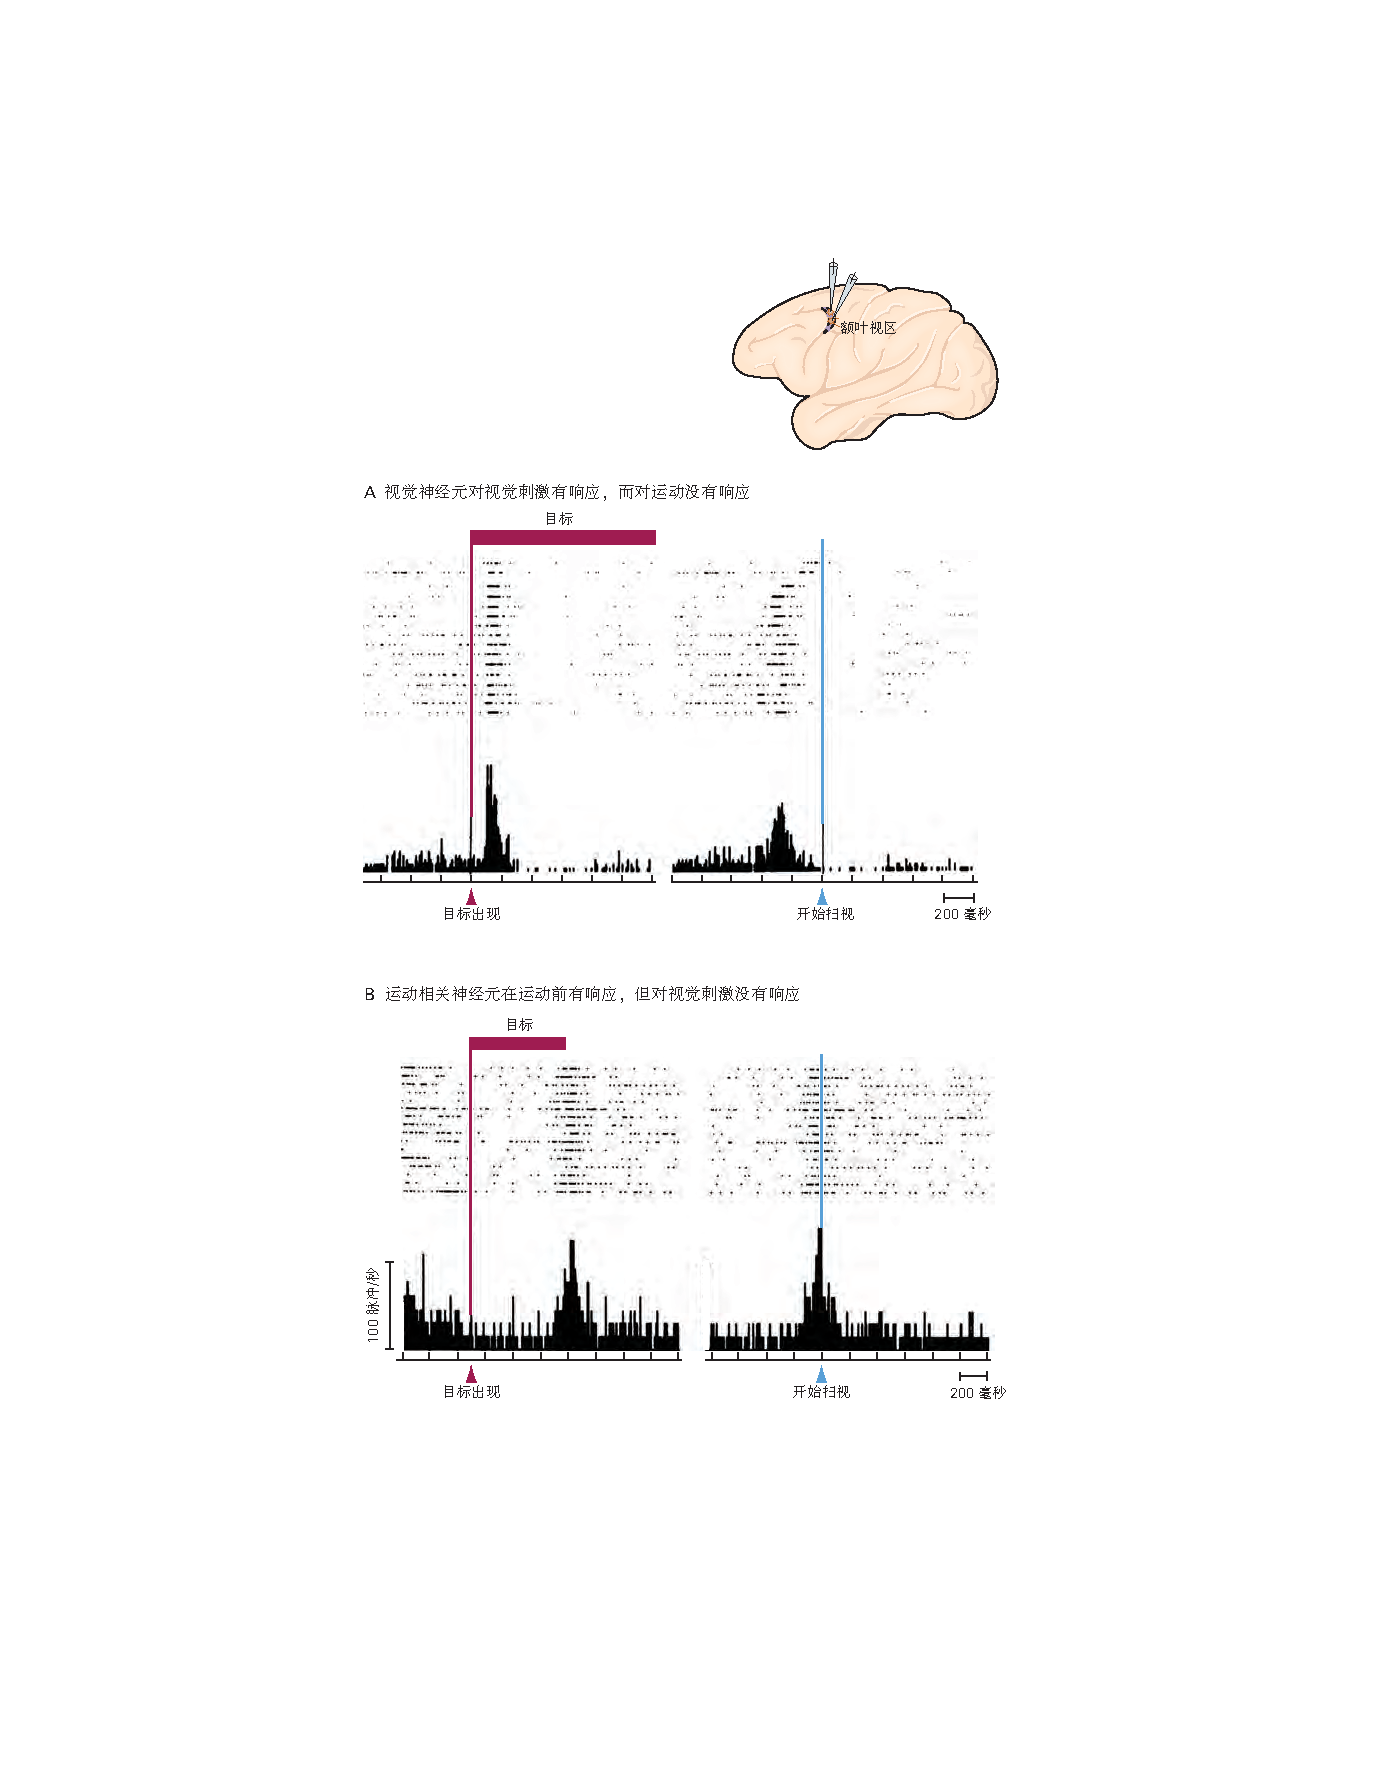
\includegraphics[width=0.8\linewidth]{chap35/fig_35_13}
	\caption{\textit{额叶视区}的视觉相关神经元和运动相关神经元\cite{bruce1985primate}。
		A. 当猴子对视野中的目标进行\textit{眼跳}时,\textit{额叶视区}视觉神经元的活动。
		同一任务的连续试验中的活动光栅图相加形成下面的直方图。
		在左侧的记录中,各个试验在刺激出现时对齐。
		突然爆发的激活与刺激密切相关。
		在右侧的记录中,试验在\textit{眼跳}开始时对齐。
		激活与\textit{眼跳}的开始并没有很好地对齐,并且在\textit{眼跳}本身开始之前就停止了。
		B. \textit{额叶视区}运动相关神经元的活动。
		每个试验的记录都按照图 A 部分进行了对齐。
		细胞对\textit{眼跳}目标(左)的出现没有响应,但在\textit{眼跳}时处于激活状态(右)。}
	\label{fig:35_13}
\end{figure}


\textit{运动相关神经元}在\textit{眼跳}运动场之前和期间会放电。
如图~\ref{fig:35_13}B~所示,与在所有\textit{眼跳}之前激活的上丘中的运动相关细胞不同,\textit{额叶视区}的\textit{运动相关神经元}仅在与猴子行为相关的\textit{眼跳}之前激活。
这些神经元,尤其是那些感受野位于视觉周边的神经元,比视觉神经元更强烈地投射到上丘。


\textit{视觉运动神经元}具有视觉和运动相关的活动,并且在视觉引导的\textit{眼跳}之前放电最强烈。
额叶视区的电刺激会引起对受刺激细胞运动场的\textit{眼跳}。
额叶视区的双侧刺激引起垂直\textit{眼跳}。


如图~\ref{fig:35_9}A~所示,\textit{额叶视区}的\textit{运动相关神经元}通过两条通路控制上丘。
一条通路是直接刺激上丘,另一条通路通过刺激\textit{尾状核}来抑制黑质,将\textit{上丘}从黑质的抑制影响中释放出来。
\textit{额叶视区}也投射到\textit{脑桥网状结构}和\textit{中脑网状结构},但不直接投射到\textit{爆发细胞}。
% 爆发细胞指 转化为肌肉信息 所指向的区域?


除了\textit{侧顶叶}之外,另外 2 个皮层区域对\textit{额叶视区}有输入,被认为在\textit{眼跳}的认知方面很重要。
辅助运动区最前端部分的\textit{辅助视区}包含编码\textit{空间信息}的神经元,而不是所需眼球运动的方向。
例如,如果向左\textit{眼跳}是在目标的右侧,则通常在右眼运动之前激活的左\textit{辅助眼区}中的神经元将在左眼\textit{眼跳}之前激活。
背外侧\textit{前额叶皮层}的神经元会在猴子向记住的目标\textit{眼跳}时放电。
激活从刺激的出现开始,并在猴子必须记住目标位置的整个时间间隔内持续进行。


% We can now understand the
我们现在可以了解这些区域的损伤对\textit{眼跳}产生的影响。
猴子\textit{上丘}的损伤只会对\textit{眼跳}系统造成短暂的损伤,因为从\textit{额叶视区}到\textit{脑干}的投射仍然完好无损。
如果上丘完好无损,动物同样可以从皮层损伤中恢复过来。
然而,当\textit{额叶视区}和\textit{上丘}都受损时,\textit{眼跳}的能力就会永久受损。
顶叶病变的主要影响是注意力缺陷。
然而,恢复后,系统可以正常工作,因为\textit{额叶视区}信号足以\textit{抑制黑质}并\textit{刺激上丘}。


仅\textit{额叶视区}的损伤会导致更细微的缺陷。
猴子\textit{额叶视区}的损伤会导致短暂的\textit{对侧空间忽视症}和逆向凝视麻痹,这些都会迅速恢复。
后一种缺陷可能反映了黑质的\textit{额叶视区}控制丧失;
这种失控意味着从黑质到上丘的持续抑制性输入没有受到抑制,上丘无法产生任何\textit{眼跳}。
最终,系统会适应,上丘会对剩余的顶叶信号做出响应。
恢复后,这些动物可以毫无困难地对视野中的目标进行\textit{眼跳},但在记忆引导的\textit{眼跳}中却有很大困难。
\textit{额叶视区}和\textit{上丘}的双侧损伤使猴子根本无法进行\textit{眼跳}。


额叶皮层受损的人很难抑制不需要的\textit{眼跳}以注意刺激。
这很容易通过要求受试者将眼球从刺激物上移开来证明,即“反\textit{眼跳}任务”。
例如,如果左侧出现刺激,则受试者应向右侧进行相同大小的\textit{眼跳}。
为此,受试者必须注意刺激,而不是将眼睛转向它,并使用它的位置来计算所需的向相反方向的\textit{眼跳}。
额叶病变患者很难抑制对刺激的不希望\textit{眼跳}。


正如我们所见,当动物注意到视觉刺激时,无论动物是否对刺激进行\textit{眼跳},猴子\textit{侧顶叶}的神经元都会活跃。
在没有\textit{额叶视区}信号的情况下,这种未分化的信号是唯一到达上丘的信号。
因此,在人类中,如果上丘对产生对刺激的注意力的顶叶信号作出响应而没有额叶-黑质控制通常会阻止响应顶叶信号的\textit{眼跳},则可以预期无法抑制\textit{眼跳}。



\subsection{\textit{眼跳}的控制可以通过经验来修改}

运动神经控制的定量研究是可能的,因为运动神经元的激活率对运动有可预测的影响。
例如,\textit{外旋运动神经元}的特定频率放电对眼睛位置和速度具有可预测的影响。


如果疾病损害动眼神经或导致眼部肌肉变弱,这种关系可能会发生变化,尽管大脑可以在某种程度上补偿这种变化。
\textit{冈特拉姆$\cdot$科默累尔}描述了一个案例,戏剧性地说明了这一点。
一名糖尿病患者的一只眼睛出现急性部分外旋神经损伤,另一只眼睛出现视网膜出血。
由于外旋神经正常的眼睛视力不佳,他通常使用新近削弱的外直肌的眼睛。
几天后,眼睛恢复了相当准确的眼球运动能力。
当弱眼被修补并且受试者试图用视力不佳的眼睛进行\textit{眼跳}时,\textit{眼跳}超出了目标。
这意味着为了补偿视觉正常眼睛的弱点,大脑增加了双眼的神经信号,导致正常运动输入的眼睛信号过大。
如图~\ref{fig:35_9}A~所示,运动响应的这种变化取决于小脑的顶核和\textit{小脑蚓体},并且是视觉系统发出信号表明之前的眼球运动不准确的结果。



\subsection{一些快速的视线转移需要协调的头部和眼睛运动}

到目前为止,我们已经描述了当头部静止时眼睛是如何移动的。
然而,当我们环顾四周时,我们的头也在移动。
必须协调头部和眼睛的运动以将中央凹引导至目标。


因为头部的惯性比眼睛大得多,所以在头部开始移动之前,注视的微小变化会驱使中央凹到达目标。
如图~\ref{fig:35_14}~所示,一个小的注视转移通常包括一个\textit{眼跳},然后是一个小的头部运动,在此期间,\textit{前庭-眼动反射}将眼睛移回新头部位置的眼眶中心。
对于较大的凝视移动,眼睛和头部同时向同一方向移动。
由于\textit{前庭-眼动反射}通常使眼睛向与头部相反的方向移动,因此必须暂时抑制反射。


\begin{figure}[htbp]
	\centering
	\includegraphics[width=0.51\linewidth]{chap35/fig_35_14}
	\caption{当头部移动时,将中央凹指向物体需要协调的头部和眼球运动。
		A. 对于轻微的视线转移,眼睛和头部会依次移动。
		目标出现300毫秒后,眼睛开始移动。
		眼动接近结束时,头部也开始移动。然后眼睛旋转回到轨道中心以补偿头部的运动。凝视记录是眼睛和头部运动的总和\cite{zee1977disorders}。
		B. 对于较大的视线转移,眼睛和头部同时向同一方向移动。
		在凝视移动接近结束时,\textit{前庭-眼动反射}恢复,眼睛开始补偿头部运动,如A部分所示,凝视变得静止\cite{laurutis1986vestibulo}。}
	\label{fig:35_14}
\end{figure}



\section{\textit{平滑跟踪}系统保持移动的目标在中央凹上}

\textit{平滑跟踪}系统通过计算目标移动的速度和以相同的速度移动眼睛来保持移动目标的图像在中央凹上。
\textit{平滑跟踪}运动的最大角速度约为每秒 100°,比\textit{眼跳}慢得多。
药物、疲劳、酒精甚至分心都会降低这些运动的质量。


\textit{平滑跟踪}和\textit{眼跳}具有截然不同的中枢控制系统。
当目标从注视中心跳开然后慢慢移回注视中心时,这种情况最为明显。
首先启动\textit{平滑跟踪}运动,因为\textit{平滑跟踪}系统具有较短的延迟并且响应周边视网膜和中央凹上的目标运动。
\textit{平滑跟踪}系统的任务不同于\textit{眼跳}系统。
它不是将眼睛尽可能快地驱动到空间中的一个点,而是必须使眼睛的速度与空间中目标的速度相匹配。
因此,如图~\ref{fig:35_6}B~所示,当目标移回注视中心时,\textit{平滑跟踪}系统会在\textit{眼跳}开始前短暂地将眼睛从目标移开。
随后的\textit{眼跳}将眼睛带到目标上。
在内侧\textit{前庭核}和\textit{舌下前置核}中发现了发出眼球速度信号以进行\textit{平滑跟踪}的神经元。
它们接收来自小脑\textit{绒球}的投射,并投射到\textit{外旋神经核}以及中脑的\textit{动眼神经核}。


\textit{绒球}和\textit{小脑蚓体}中的神经元传输和\textit{平滑跟踪}相关的眼速信号。
如图~\ref{fig:35_15}~所示,这些区域接收由脑桥背外侧核中继的大脑皮层信号。
因此,背外侧脑桥的损伤会破坏同侧的\textit{平滑跟踪}。


\begin{figure}[htbp]
	\centering
	\includegraphics[width=0.87\linewidth]{chap35/fig_35_15}
	\caption{猴子\textit{平滑跟踪}眼球运动的皮层通路。
		大脑皮层处理有关视野中运动的信息,并通过\textit{背外侧脑桥核}、\textit{绒球}和\textit{小脑蚓体}以及\textit{前庭核}将其发送到动眼神经元。
		\textit{平滑跟踪}的启动信号可能部分源自\textit{额叶视区}。}
	\label{fig:35_15}
\end{figure}


猴子的\textit{平滑跟踪}系统有 2 个主要的皮层输入。
一种起源于\textit{颞上沟}、\textit{中颞}和\textit{上颞内侧区}的运动敏感区。
另一个来自\textit{额叶视区}。


\textit{中颞}和\textit{上颞内侧区}因其位于\textit{夜猴}(一种\textit{新大陆猴})的无沟皮层中而得名。
在人类和\textit{旧大陆猴}中,这些区域位于枕叶和顶叶交界处的\textit{颞上沟}。
\textit{中颞}和\textit{上颞内侧区}的神经元\textit{计算目标的速度}。
当眼睛加速以匹配目标的速度时,目标在视网膜上的运动速度会降低。
% 眼睛在动了,目标在视网膜上就可以不动
随着视网膜图像速度的降低,\textit{中颞}神经元(其活动发出视网膜图像运动信号)停止放电,即使目标继续在空间中移动也是如此。
即使目标短暂消失,\textit{上颞内侧区}的神经元也会继续放电。
% “这些神经元”指的是中颞和上颞内侧区的神经元?
这些神经元可以访问一个过程,该过程将\textit{目标在视网膜上移动的速度}和\textit{眼睛移动的速度}相加,以计算\textit{目标在空间中的速度}。


\textit{中颞}或\textit{上颞内侧区}的损伤会破坏受试者对在受损皮层区域代表的视野区域中移动的目标做出响应的能力。
无论目标位于视网膜上的哪个位置,后一区域的病变也会减少向病变一侧的\textit{平滑跟踪}运动。


这 2 个运动选择区域提供感官信息来指导跟踪运动,但可能无法启动它们。
任一区域的电刺激都不会启动\textit{平滑跟踪},但可以影响跟踪运动,加速同向跟踪并减慢反向跟踪。
正面视野对于发起跟踪可能更为重要。
该区域的神经元会随着同向的\textit{平滑跟踪}而发射。
\textit{额叶视区}的电刺激启动同向跟踪,而该区域的病变减少但不消除\textit{平滑跟踪}。


在人类中,跟踪路径沿途任何地方的中断,包括皮层、小脑和脑干区域水平的损伤,都会阻止足够的\textit{平滑跟踪}眼球运动。
相反,使用有缺陷的\textit{平滑跟踪}运动(速度小于目标速度)和小\textit{眼跳}的组合来跟踪移动目标。
脑干和小脑病变的患者不能跟踪向病变一侧移动的目标。


包括运动敏感区域在内的顶叶缺陷患者有 2 种不同类型的缺陷。
第一个是方向性缺陷,类似于患有\textit{上颞内侧区}病变的猴子:
无法跟踪向病变一侧移动的目标。
第二种是类似于患有中颞区病变的猴子的视黄质缺陷:
无论运动方向如何,都存在对仅限于病变对面的视觉半视野的刺激的\textit{平滑跟踪}的损害。



\section{聚散系统将眼睛对齐到不同深度的目标上}

\textit{平滑跟踪}和\textit{眼跳}系统产生\textit{双眼同向运动}:
双眼以相同的方向和相同的速度移动。
相反,聚散系统产生眼睛的非\textit{双眼同向运动}。
当我们注视一个离我们很近的物体时,我们的眼睛会聚或向对方转动;
如图~\ref{fig:35_16}~所示,当我们看一个更远的物体时,它们会发散或旋转远离彼此。
这些分离运动确保物体的图像落在 2 个视网膜的中央凹上。
视觉系统利用左右视网膜位置的细微差异或视网膜视差来产生深度感,而聚散运动则消除中央凹处的视网膜视差。


\begin{figure}[htbp]
	\centering
	\includegraphics[width=0.7\linewidth]{chap35/fig_35_16}
	\caption{聚散运动。
		当眼睛注视远处的山时,山的影像位于中央凹,而前方树木的影像占据不同的视网膜位置,产生双重影像的感知。
		当观察者转而注视树时,聚散系统必须将每只眼睛向内旋转。
		现在,树的图像在 2 个中央凹上占据相似的位置,并被视为一个物体,但山的图像在视网膜上占据不同的位置,看起来是双重的。}
	\label{fig:35_16}
\end{figure}


聚散度仅是水平直肌的功能,因为两只眼睛是水平而非垂直移位的。
用于近场观看的眼睛会聚是通过同时增加内侧直肌的张力和降低外侧直肌的张力来使眼睛会聚来实现的。
相反,远距离观察是通过降低内直肌的张力和增加外直肌的张力来实现的。


在任何给定时间,整个视野都不会聚焦在视网膜上。
当我们看近处的东西时,远处的物体是模糊的。
当我们看远处的东西时,近处的物体是模糊的。
当我们希望聚焦在视野中较近平面中的物体时,动眼神经系统收缩睫状肌,从而改变晶状体的曲率半径。
这个过程称为适应。
随着年龄的增长,由于晶状体硬度增加,调节能力下降;
然后需要老花镜来聚焦近距离的图像。


住宿和聚散度是相关的。
调节是由图像的模糊引起的,每当调节发生时,眼睛也会聚集。
相反,视网膜差异会引起聚散,每当眼睛会聚时,也会发生调节。
同时,瞳孔会暂时收缩以增加焦点的景深。
调节、聚散和瞳孔收缩的相关现象构成了近距离响应。
调节和聚散由动眼神经核区域的中脑神经元控制。
该区域的神经元在聚散、调节或两者同时放电。



\section{要点}

1. 动眼神经系统为临床医生和科学家提供了了解神经系统的宝贵窗口。
患有动眼神经缺陷的患者可能会出现复视等令人担忧的症状,这些症状会使他们迅速寻求医疗帮助。
对动眼神经系统有透彻了解的医生可以在床边描述和诊断大多数动眼神经缺陷,并根据眼球运动的神经解剖学和神经生理学定位大脑内的病变部位。


2. 眼球运动的目的是在眼眶中转动眼球,以便将中央凹(视网膜上具有最佳敏锐度的区域)引导到视觉场景中最感兴趣的点,然后保持图像稳定。


3. 6 块肌肉共同作用来移动每只眼睛。
这些眼部肌肉分为 3 对。
外直肌水平外展眼球,内直肌内收眼球。
旋转眼肌在垂直方向和扭转方向上移动眼睛。


4. 眼外肌的运动神经元位于 3 个脑干核团中。
脑桥中的\textit{外旋神经核}包含外直肌的神经元。
其他动眼神经元位于中脑:滑车核包含上斜神经元,动眼神经核包含内侧、上、下直肌和下斜肌的运动神经元。
收缩瞳孔和抬高眼睑的神经元也位于动眼神经核中。


5. 有 6 种不同类型的眼球运动,具有不同的控制系统:(1)\textit{眼跳}快速将中央凹转移到新的视觉目标。
(2)\textit{平滑跟踪}运动将移动物体的图像保留在中央凹上。
(3)聚散运动使眼睛向相反的方向旋转,以便无论距离多远,感兴趣的物体的图像都位于 2 个中央凹上。
(4)\textit{前庭-眼动反射}在短暂、快速的头部运动期间将图像保持在视网膜上。
(5)视动运动在持续或缓慢的头部运动期间保持图像静止。
(6)注视是在头部不动时,在注视过程中保持眼睛静止的主动过程。


6. 眼肌神经元的放电模式结合了编码眼睛位置和速度的独立信号。
产生水平\textit{眼跳}速度信号的神经元位于\textit{脑桥旁正中网状结构}中,该速度信号整合在内侧前庭核和舌下核前置核中以提供位置信号。


7. 中脑网状结构为垂直和扭转眼球运动以及聚散眼球运动提供位置和速度信号。


8. 上丘中的\textit{眼跳}前爆发神经元将所需的位移信号投射到网状结构。
这些神经元被来自黑质的\textit{$ \gamma $-氨基丁酸能}投射抑制,并被来自\textit{额叶视区}和后顶叶皮层的投射兴奋。
来自\textit{额叶视区}的运动信号激发尾状核,然后尾状核抑制黑质,使\textit{眼跳}发生。


9. 后顶叶皮层向上丘投射注意信号,不区分注意和运动。


10. 大多数大的凝视转移都涉及头部运动和眼球运动。
因为眼睛比头移动得快,所以它通常先到达目标。
\textit{前庭-眼动反射}通过以与头部运动的速度相反的速度驱动眼睛来保持眼睛在目标上。


11. 小脑根据视觉反馈校准眼球运动并调节学习过程,使它们随着时间的推移保持准确。


12. \textit{平滑跟踪}是由一个网络驱动的,该网络包括内侧前庭核、小脑绒球、背外侧脑桥核,以及在一些猴子的\textit{颞上沟}中发现的 2 个运动选择区域:\textit{中颞}和\textit{上颞内侧区}。
人脑中的同源区域位于顶枕叶交界处。
额叶视区的跟踪区域启动\textit{平滑跟踪}运动。


13. 尽管眼球运动的运动程序已广为人知,但该领域的大部分生理学研究都是通过猴子对光点进行定向\textit{眼跳}来完成的。
我们对探索视觉世界时自由选择\textit{眼跳}目标的神经机制知之甚少。
这个位于认知和运动控制交叉点的问题是神经科学中最大的未知数之一,将成为未来动眼神经研究的中心。




